\documentclass{article}
% basics
\usepackage{amsfonts}
\usepackage{enumitem}
\usepackage{float}
\usepackage{graphicx}
\usepackage{hyperref} 
\usepackage[labelfont=bf]{caption}
\usepackage{geometry}
\geometry{margin=4cm}

\newtheorem{theorem}{Theorem}
\newtheorem{lemma}[theorem]{Lemma}
\newtheorem{corollary}{Corollary}[theorem]

% unique math expressions:  
\usepackage{amsmath}
\DeclareMathOperator*{\andloop}{\wedge}
\DeclareMathOperator*{\pr}{Pr}
\DeclareMathOperator*{\approach}{\longrightarrow}
\DeclareMathOperator*{\eq}{=}

% grey paper
\usepackage{xcolor}
% \pagecolor[rgb]{0.11,0.11,0.11}
% \color{white}

% embedded code sections
\usepackage{listings}
\definecolor{codegreen}{rgb}{0,0.6,0}
\definecolor{codegray}{rgb}{0.5,0.5,0.5}
\definecolor{codepurple}{rgb}{0.58,0,0.82}
\lstdefinestyle{mystyle}{
    commentstyle=\color{codegreen},
    keywordstyle=\color{magenta},
    numberstyle=\tiny\color{codegray},
    stringstyle=\color{codepurple},
    basicstyle=\ttfamily\footnotesize,
    breakatwhitespace=false,         
    breaklines=true,                 
    captionpos=b,                    
    keepspaces=true,                 
    numbers=left,                    
    numbersep=5pt,                  
    showspaces=false,                
    showstringspaces=false,
    showtabs=false,                  
    tabsize=2
}

\lstset{style=mystyle}

\begin{document}
\author{Yosef Goren}
\title{Internet Networking 236341 - Homework 2}
\maketitle
\tableofcontents

\section{BGP Business Relations}
In this question we are assuming the export policy:
\begin{enumerate}[label=\textbf{\Roman*.}]
    \item If the route is via a customer - advretize to all neighbors.
    \item Advresize all routes to all customers.
    \item Otherwise - do not advretize.
\end{enumerate}
We are also assuming that the import policy is to accept all incoming routes.

\subsection{\texttt{(6,3,4,7)}}
The route is possible in terms of the export policy:\\
AS4 sees the route $4\rightarrow 7$ and due to rule I - it advretizes
it to AS3.\\
AS3 sees possbile route $3\rightarrow 4\rightarrow 7$, and due to rule II,
it advretize it to AS6.\\
Hence AS6 has the route $6\rightarrow 3\rightarrow 4\rightarrow 7$,
so it is possible in terms of the export policy.

\subsection{\texttt{(6,3,4,5)}}
The route is not possible, AS5 isn't a costumer 
of AS4, so the route through AS4 to AS5 will not be exported 
to AS3, and the route isn't possible.

\subsection{\texttt{(6,7,5)}}
This route is not possible.\\
Since AS6 is not a customer of AS7 (rule II not satisfied), and AS5 is not a customer
of AS7 (rule I not satisfied) - then AS7 will not advretize the route $7\rightarrow 5$
to AS6, so it has not way of know that this route exists.

\subsection{\texttt{(3,1,4)} - $\pi$}
The route is possible.\\
AS1 sees the route $1\rightarrow 4$,
and since AS4 is it's customer (rule I), it will advretize this route to AS3 -
hence AS3 knows about the route $3\rightarrow 1\rightarrow 4$.

\subsection{\texttt{(2,4,5)}}
This route is not possible.\\
AS4 is not a provider for neither AS2 nor AS5 - hence
it will not advretize the route $4\rightarrow 2$ to AS5.\\
So AS5 will not know about this route.

\subsection{\texttt{(4,7,5)}}
This route is not possible.\\
Since to AS7 - neither AS4 nor AS5 are customers, it will not advretize
the route $7\rightarrow 4$ to AS5, and so AS5 does not know about the route $5\rightarrow 7\rightarrow 4$.
\section{ICMP}
\subsection{ICMP types and codes}
\begin{enumerate}[label=\textbf{\alph*.}]
    \item The router sends an ICMP Time Exceeded packet to
    with \texttt{type=11} and \texttt{code=0} which means it is due to TTL running out.
    \item The router sends an ICMP Destination Unreachable packet,
    with \texttt{type=3} and \texttt{code=4} which means that fragmantation was required
    but not allowed due to the DF flag.
    \item The router sends an ICMP Destination Unreachable packet,
    with \texttt{type=3} and \texttt{code=1} which means the destination network is unreachable.
    \item The router sends an ICMP Destination Unreachable packet,
    with \texttt{type=3} and \texttt{code=3} which means
    the destination port is unreachable.
    \item It will send a packet with \texttt{type=5} and \texttt{code=0}
    which indicates that a packet was forwareded but the existing routing is used was not optimal in
    the sense that it should have been routed through the same LAN.
    \item The router will return an ICMP echo reply packet
    which has \texttt{type=0}, \texttt{code=0}.
    \item The router sends an ICMP Destination Unreachable packet,
    with \texttt{type=3} and \texttt{code=0} which
    means that the destination address could not be reached.
\end{enumerate}
\subsection{MTU discovery}
MTU is the Maximum Transmission Unit,
which is a number (in bytes) that describes the maximal size of a packet
that will be sent.\\
MTU discovery is a process where on a specific socket - the two communicating
parties attempt to find the MTU for the links that connect them - so
they can send packets with the optimal size in their communication.\\

MTU discovery is done by attempting different message sizes (and \texttt{DF=1}) and seeing which
are capable of passing and which do not return or result with an 'ICMP could not Fragment' - which
means the packet was too large.
A failiure indicates the packet size is larger than the MTU while 
a success indicates the packet size is smaller or equal to the MTU.
To accelerate this process a binary search algorithm can be used.

\subsection{ICMP and IP}
ICMP is the Internet Control Message Protocol while IP is Internet Protocol.\\
The ICMP protocol enables the IP protocol to work, by transfering
metadata about how IP messages are moving through the network (such as in the examples in the first
part of the question).\\
It is also somewhat circular as ICMP packets are built upon the IP headers,
while the routers and hosts that transfer IP packets relay on the ICMP
protocol to be configured properly.
\section{Stiner Tree}
\subsection{SPT}
Our SPT tree is:
\begin{center}
    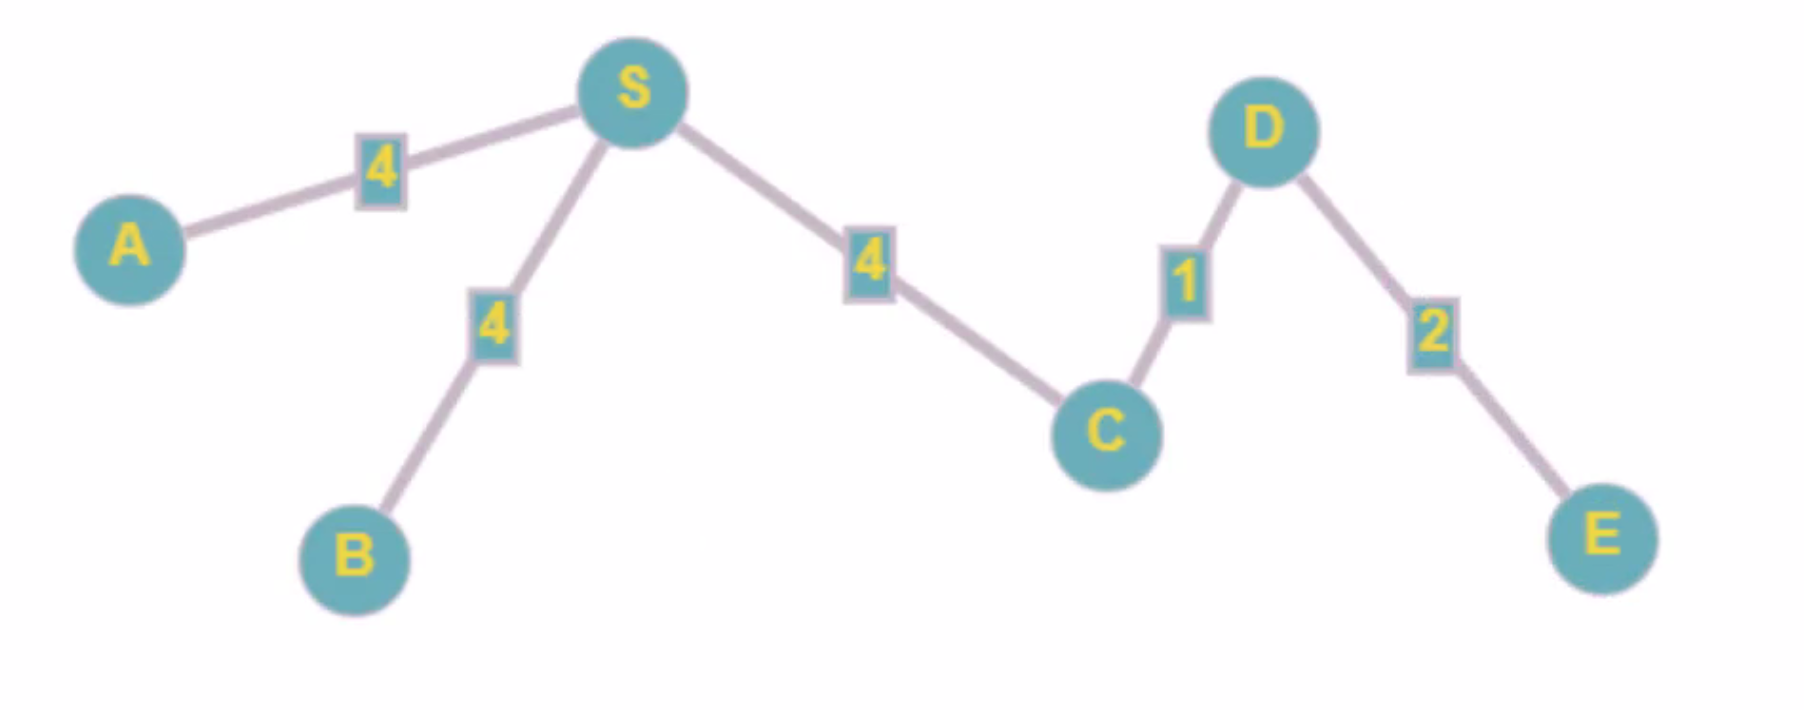
\includegraphics[width=0.6 \textwidth]{resources/q3-1.png}\centering
\end{center}
And it's weight is 15.\\
The maximal weight of a path from the source is that of the path to E,
which is 7.

\subsection{Huristic Algorithm}
The resulting clique is:
\begin{center}
    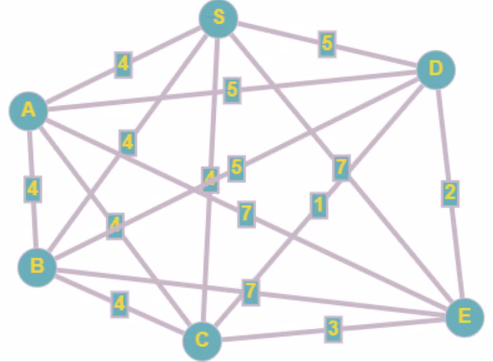
\includegraphics[width=0.6 \textwidth]{resources/q3-3.png}\centering
\end{center}
And a minimum spanning tree we have found for it is:
\begin{center}
    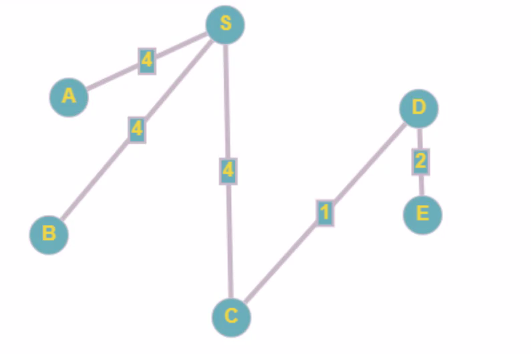
\includegraphics[width=0.6 \textwidth]{resources/q3-4.png}\centering
\end{center}
Where the weight of the maximum path is 7. 

\begin{figure}
    \begin{center}
        
\includegraphics[width=0.6 \textwidth]{resources/q3-2.png}\centering
    \end{center}
    \caption{Algorithms...}
\end{figure}


\subsection{Stiener Tree}
The Stiener Tree is:
\begin{center}
    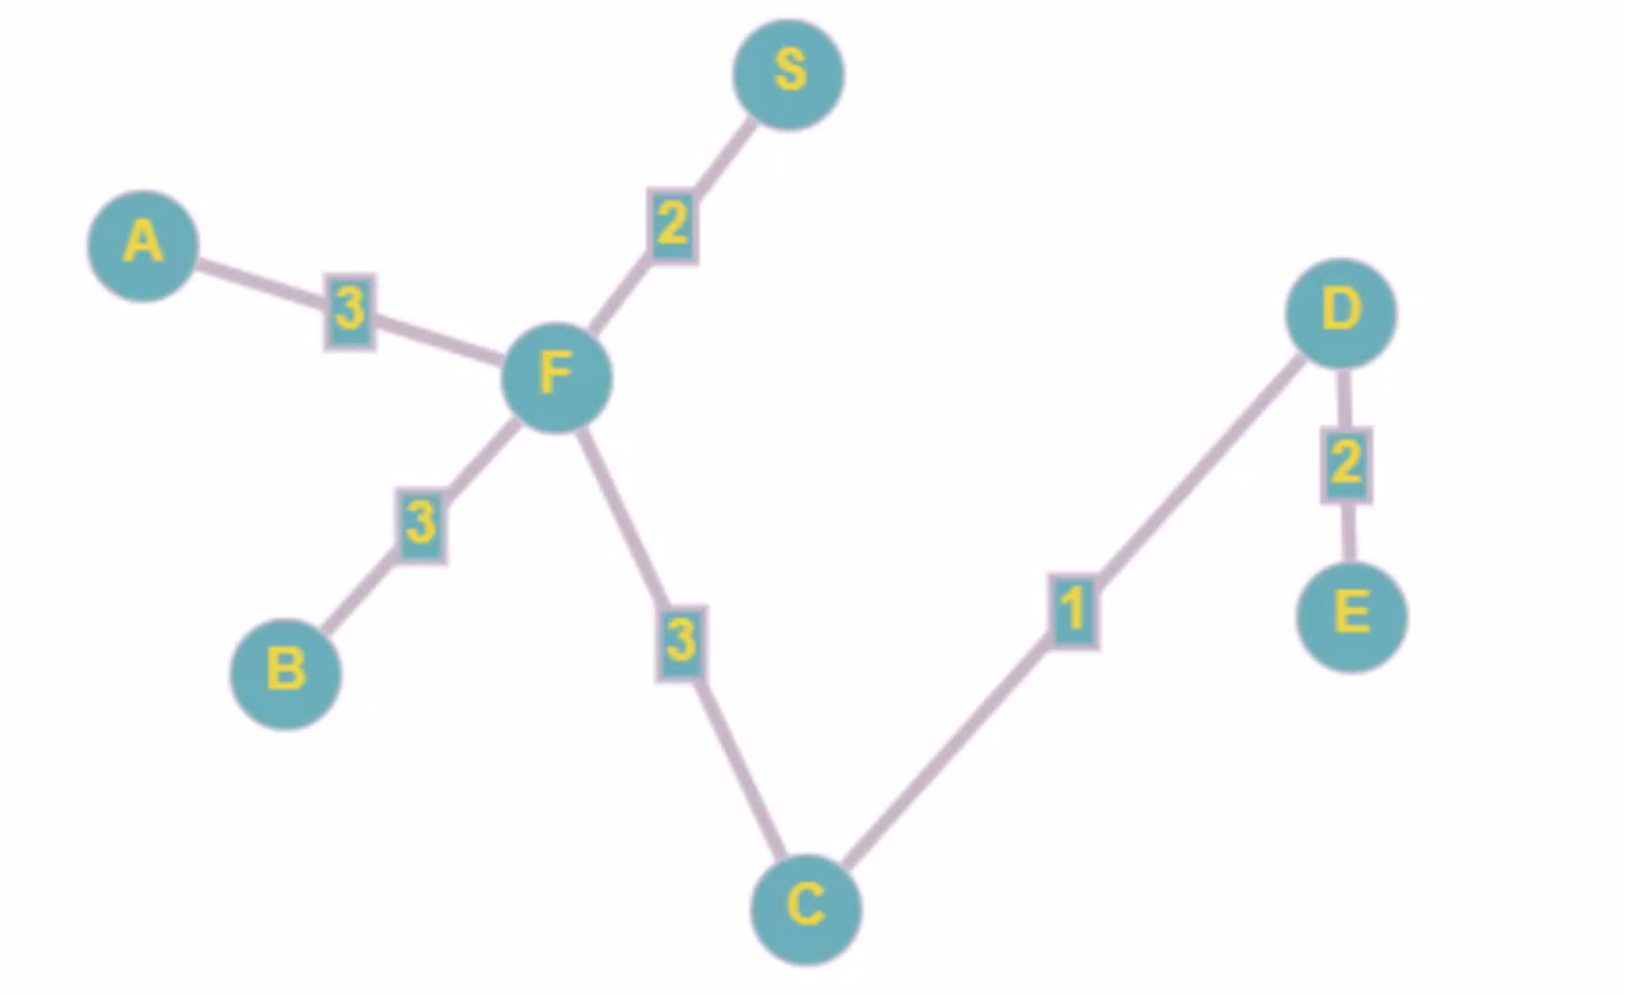
\includegraphics[width=0.6 \textwidth]{resources/q3-5.png}\centering
\end{center}
It's weight is 14, the maximal path weight is 8 
- that path is $S\rightarrow F\rightarrow C\rightarrow D\rightarrow E$.

\subsection{Stiner Vs Huristic}
The Huristic trees are (much) easier to find
\footnote{finding a stiner tree is an NP-Complete problem},
and in some cases the might also have
have a shorter longest path between two nodes (such as we can see in the prior example),
and the advantage of the Stiner trees is that they guarantee (by definition)
that they have the lower total weight.

\end{document}